% !TEX root = ../thesis.tex
% !TeX spellcheck = en_US

In this last chapter, the work is summarized and future work is presented.

The presented \emph{hybrid routing algorithm} combines graph-based with geometric routing and, furthermore, determines shortest paths between arbitrary source and destination locations.
The geometric routing component is based on visibility graphs containing only edges between vertices that are visible to each other.
Edges in visibility graphs are therefore the shortest connection between two vertices, a useful property for finding general shortest paths.
Generating a routable visibility graph is one core task of the hybrid routing algorithm.

Merging road edges from the input dataset into the visibility graph is the second core task of the hybrid routing algorithm.
During this step, intersecting road and visibility edges are split and connected to allow paths to alternate between these two types of edges.

The graph-based routing component consists of a normal graph-based algorithm, A* in this case, and may use speedup techniques.
The source and destination locations are added and connected to the graph, as far as they are not represented by existing vertices, which allows the determination of shortest paths between arbitrary locations.
	
\section{Future work}
\label{sec:future-work}

	Even though the presented algorithm works as intended, some problems are known and a certain potential for further enhancements exists.
	This section discusses these problems and potential solutions, lists additional technical enhancements and outlines additional functionalities the hybrid routing algorithm might benefit from.

	\subsection{Known problems}
		% Overall: Speed up visibility edge generation for initial import + routing
		It might not be a severe problem to all agent-based models and scenarios, but the graph generation and routing performance offers potential for improvement.
		This can happen by optimizing the current implementation or implementing a different graph generation algorithm.
		
		The first approach might use better data structured for vertices and obstacles.
		In the current implementation, for every vertex, every other vertex in the dataset is considered a potential neighbor and then filtered out using e.g. valid angle and shadow areas.
		Using a spatial index to query vertices in certain areas might increase performance since not all vertices need to be checked.
		However, any additional data structure also introduces additional overhead and might only be beneficial for datasets of a certain size.
		Therefore, the usefulness of this approach needs to be tested and evaluated.
		
		The second approach is a complete reimplementation of the edge creation.
		Such a reimplementation might use approaches mentioned in \Cref{subsec:related-work:visibility-graph,subsec:suitablilty-edge-creation-approaches}, which showed promising sub-quadratic runtime complexities.
		
		\begin{wrapfigure}{r}{0.35\textwidth}
%			\vspace{-0.5\baselineskip}
			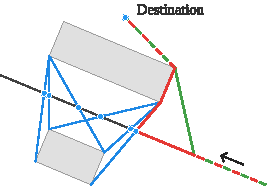
\includegraphics[width=\linewidth]{images/qgis-future-work-connectivity-problem}
			\caption[Example connectivity problem.]{Connectivity problem in case of too few visibility edges. The green path might be the expected result, but the red path is the determined shortest path.}
			\label{fig:connectivity-problem}
			\vspace{0.5\baselineskip}
			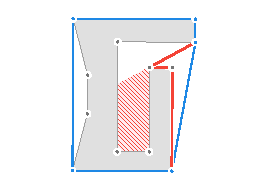
\includegraphics[width=\linewidth]{images/qgis-future-work-convex-hull-problem}
			\caption[Illustration of unreachable areas in concave polygons.]{Concave polygons do not always contain all necessary edges (red) but only those edges connecting the convex hull (blue). Some regions are therefore unreachable (red marked area).}
			\label{fig:convex-hull-problem}
		\end{wrapfigure}
				
		% Connection to roads based on the hope that there are many visibility edges (in the end the vast number of edges creates a irregular grid like structure even though v-edges are not connected to each other)
		In datasets with very few obstacles, the connectivity between road and visibility edges may be reduced due to a sparse visibility graph, meaning edges are missing to switch between road and visibility edges properly.
		\Cref{fig:connectivity-problem} illustrates this:
		the green expected path cannot be used due to missing edges, which leads to the suboptimal red route.
		Forcing the creation of additional edges, e.g. by connecting all vertices of roads or splitting roads at certain distances, might solve this problem.
		
		Another problem arises with \enquote{islands} inside of obstacles, for example, an actual island inside a lake that is reachable via an edge representing a pedestrian bridge.
		Even though the hybrid routing algorithm creates edges inside the island, it might also create edges inside the lake.
		Handling inner rings of (multi-)polygons is therefore needed to correctly navigate within islands of obstacles.
		
		% Convex hull filtering might lead to problems for obstacle part not directly visible to outside (like a cave). Concave hull filtering might be the correct solution.
		One optimization of the graph generation process is filtering vertices by convex hulls as introduced in \Cref{subsubsec:convex-hull}.
		However, this optimization only works for polygons with no hidden vertices, i.e. vertices that are theoretically reachable but inside the obstacle and not visible to the outside.
		\Cref{fig:convex-hull-problem} illustrates the problem with the red marked area, which is not reachable when only vertices of the convex hull are connected.
		The red edges are necessary to create a shortest path from and to the area within the obstacle.
		
		% Point like barriers (e.g gate on a road) have nearly no effect → generate orthogonal line-barrier or remove all visibility edges within a radius or something
		A different type of problem arises with road vertices containing attributes that make them a punctual barrier.
		In OSM, this is for example the case for a node being part of a road and containing the tag \texttt{barrier=gate}.
		In reality, however, such gates and entrances are not only punctual features but often belong to a wall or fence.
		These linestring barriers are not relevant for purely graph-based routing and therefore do not always exist in OpenStreetMap.
		These line-based barriers are very important for the hybrid routing algorithm to ensure correct routing results.
		Without these barriers, the routing will avoid the road, due to the barrier-attribute, but instead might use a visibility edge next to the road.
		Adding the missing linestring barriers to the underlying dataset is the ideal solution but algorithmic approaches might also exist to infer these linestrings automatically.
		
	\subsection{Technical and performance enhancements}
		
		Future work might also consider technical enhancements, improving the implementation and eventually improving routing results and performance.
	
		% kD-tree implementations: MARS implementation expensive, NTS implementation only works on classes (MARS stuff often struct) + not supports multiple nodes at same location. Own implementation specifically for points might help
		The \texttt{HybridVisibilityGraph} class uses a k-d tree as a spatial index for the nodes in the graph, which allows fast queries to find existing nodes at given coordinates.
		This operation is used multiple times when answering routing queries to add locations to the graph.
		Even though the data structure is suitable for this task, there are some technical reasons why this can be enhanced.
		First, the used k-d tree implementation of MARS internally uses an array-based stack, which is resized multiple times when answering queries to the k-d tree and therefore significantly reduces its performance.
		Second, the NTS also offers a generic k-d tree implementation that only works on classes and only allows unique values, i.e. one node per coordinate.
		Unfortunately, both criteria are not fulfilled since each node is a \texttt{struct} and multiple nodes might exist per coordinate.
		Working around these problems, enhancing an existing implementation or choosing a different index structure will likely improve the performance of routing queries.
		
		% Splitting vertices by their valid angle area might simplify implementation + speeds up graph generation since angle area checks are very very fast.
		In the current implementation, visibility neighbors are determined for each input vertex, then sorted into bins based on the obstacle neighbors of the vertex and finally output vertices are created per bin.
		This approach of determining visibility neighbors first and then splitting the vertices introduces a certain complexity to the code.
		Splitting vertices based on their obstacle neighbors \emph{before} determining the visibility neighbors makes handling of valid angle areas easier and sorting the visibility neighbors into bins will no longer be necessary.
		Not only the code complexity but the overall performance might benefit from such a refactoring as well.
		
		Next to performance enhancements in terms of the required time, memory usage can also be improved.
		As illustrated in \Cref{subsec:memory-consumption}, merging the road graph led to the most significant increase in memory usage.
		Further analysis needs to take place to find the steps responsible for this increase in memory.
		One possible enhancement is the combination of data structures and indices in the \texttt{HybridVisibilityGraph}.
		However, the number of nodes and edges are likely the cause of the high memory usage, which can be reduced by the following approach.
		
		% Reduce edge-count e.g. with approaches described in "A Modular Routing Graph Generation Method for Pedestrian Simulation" (Kielar, 2016). This might not speed up anything, though since the visibility calculation is based on vertices. However, this might result in fewer road-segments and faster connection of new edges (which is not that slow anyway)
		The number of edges in the hybrid visibility graph is very high due to the functioning of visibility edges but also due to merged road edges.
		Approaches exist to reduce the number of edges in a routing graph with little effect on the route quality \cite{aumann-reducing-routing-graph}, which will speed up graph generation and routing but reduce the memory consumption.

	\subsection{Additional functionalities}
		
		Possible future work on the hybrid visibility approach might not only improve the performance and solve existing issue but might also introduce new useful functionalities.
		
		% Taking road restrictions into account (tags as well as size)
		One possible feature is the consideration of road tags.
		On the one hand, this includes the usage attributes in the weighting function, such as legal restrictions for pedestrian traffic.
		On the other hand, road attributes can be used to find unrealistic visibility edges.
		For example, a visibility edge crossing an eight-lane primary road can be removed since real pedestrians, at least under normal circumstances, will probably not cross such roads.
		Knowing the size of the road can also help to identify visibility edges lying within the area of that road, which means these edges are not realistically usable by pedestrians in the real world.
		Road attributes can therefore enhance the quality of the routes.
		
		% 3D data: Handling OSM level-tags (vertical relation between roads)
		At least in OpenStreetMap, the third dimension, meaning the vertical orientation of features, is specified by specific attributes.
		This 3D data is currently not supported but would enhance routing in densely built-up urban scenarios with bridges, tunnels or multi-story datasets.
		
		% Adding attributes to edges (e.g. when visibility edge goes over grass area → surface=grass to edge)
		Next to evaluating existing attributes, added attributes on visibility edges can be used by the underlying graph-based algorithm for more accurate routing and also for additional path information for potential end-users.
		For example, visibility edges traversing grass areas can be augmented with an attribute such as \texttt{surface=grass}.
		Having attributes on visibility edges enables the routing algorithm to prefer or avoid edges, e.g. by their surface conditions.
		
		% Storing graph in a format that keeps the same-location-nodes + additional angle information
		The current implementation works solely in the main memory, which means the import has to be performed for every execution of a simulation.
		Storing the hybrid visibility graph to disk detaches the graph generation from its use.
		
		% Parallel usage of routing
		When using the hybrid visibility graph, routing requests might change the underlying graph by adding new nodes and edges.
		Even though this only adds new possibilities to the routing, parallel routing requests are currently not explicitly supported and might cause problems and unexpected routing results.
		Allowing parallel routing requests helps autonomous agents to determine optimal paths independently.
		Possible strategies to introduce parallelism need to be determined.
		
		% Dynamic changes in obstacles, meaning add, remove or change existing obstacles. Visibility edges need to be re-calculated, but not all → which ones?
		The presented hybrid visibility graph is static, meaning the data does not change.
		However, it is already possible to dynamically and temporarily add and connect nodes to the graph.
		Extending this into the possibility of dynamically changing the existing data of the graph enables the hybrid visibility graph to be used in numerous additional scenarios in which the environment dynamically changes.
		This is particularly interesting for agent-based simulations, e.g. in a flooding scenario where the flooded area changed over time, but also for real-world applications taking for example real-time traffic data and construction sites into account.
		
\section{Conclusion}

	The presented hybrid routing algorithm enables the determination of shortest paths between arbitrary locations by using a combination of an existing road network with visibility edges to cross open areas.
	An evaluation of the implementation showed expected results for the following three main aspects regarding performance and route quality.
	
	First, the overall performance shows the expected inherent quadratic time complexity due to the visibility graph creation.
	Effective optimizations were able to reduce the required processing time significantly.
	Second, the route quality does benefit from edges covering open spaces and the routes did become shorter and more realistic considering expected routes real pedestrians would likely choose.
	Agent-based models simulating human behavior can benefit from this increased realism of the routes.
	In contrast to the hybrid routing algorithm, purely graph-based routes showed a lower quality with longer routes and sometimes large detours, especially in rural areas with larger open spaces and a less dense road network.
	And third, the data quality significantly impacts the route quality.
	Missing or wrong data leads to inaccurate or routes that are unusable in the real world.
	
	The presented algorithm has the potential for enhancements and might be part of future work.
	However, I am convinced that use cases in agent-based simulations and real-world applications exist in which the hybrid routing algorithm is beneficial for the quality of the determined routes.